\chapter{Fluid Modelling of Plasmas and Sheaths}
\label{ch:fluid}

Earlier chapters track the full distribution functions $f_{\mathrm{e}}(\mathbf{r},\mathbf{v},t)$ and $f_{\mathrm{i}}(\mathbf{r},\mathbf{v},t)$ under the Boltzmann equation, resolving non-Maxwellian tails, trapped populations and the fine structure of the ion energy distribution at a wall. That completeness is expensive: a kinetic solve of the plasma-sheath system is a high-dimensional phase-space problem repeated for every density, temperature and bias explored, and inverting a measured ion energy flux $\Gamma_{E}$ onto bulk plasma parameters may need thousands of forward evaluations, more than a kinetic solver can sustain inside an optimisation loop or Markov-chain sampler. Fluid models close this gap: velocity moments of the Boltzmann equation yield a hierarchy of macroscopic conservation laws for density, momentum and energy that, once truncated by a closure hypothesis, reduce to a small system of differential equations in space and time alone. This chapter develops that hierarchy, catalogues common closures, derives the classical fluid sheath model and the Bohm criterion it implies, discusses where the fluid approximation fails near the sheath edge, specifies the boundary conditions coupling a fluid presheath to the sheath, and connects the formalism to the forward-modelling needs of the ion energy flux inversion at the centre of this monograph.

\section{Moments of the Boltzmann Equation}
\label{sec:moments}

\subsection{The kinetic starting point}

For each species $s\in\{\mathrm{e},\mathrm{i}\}$, with mass $m_s$, charge $q_s$ and distribution function $f_s(\mathbf{r},\mathbf{v},t)$ normalised so that $n_s(\mathbf{r},t)=\int f_s\,\mathrm{d}^3v$, the Boltzmann equation reads
\begin{equation}
\frac{\partial f_s}{\partial t} + \mathbf{v}\cdot\nabla f_s + \frac{q_s}{m_s}\left(\mathbf{E}+\mathbf{v}\times\mathbf{B}\right)\cdot\nabla_{\mathbf{v}} f_s = C_s[f_s],
\label{ch12-eq:boltzmann}
\end{equation}
where $C_s[f_s]$ is the collision operator, covering elastic Coulomb collisions, charge exchange, ionisation and recombination. The fluid approach integrates this against successive powers of $\mathbf{v}$, the procedure underlying the first-principles derivation of the Bohm criterion \cite{ref0670}; every fluid sheath model below is a truncation of this hierarchy.

Define the moments
\begin{align}
n_s(\mathbf{r},t) &= \int f_s\,\mathrm{d}^3v, \label{eq:mom0}\\
n_s\mathbf{u}_s(\mathbf{r},t) &= \int \mathbf{v}\,f_s\,\mathrm{d}^3v, \label{eq:mom1}\\
\mathsf{P}_s(\mathbf{r},t) &= m_s\int (\mathbf{v}-\mathbf{u}_s)(\mathbf{v}-\mathbf{u}_s)\,f_s\,\mathrm{d}^3v, \label{eq:mom2}\\
\mathbf{q}_s(\mathbf{r},t) &= \frac{m_s}{2}\int (\mathbf{v}-\mathbf{u}_s)\,|\mathbf{v}-\mathbf{u}_s|^2\,f_s\,\mathrm{d}^3v, \label{eq:mom3}
\end{align}
the density, mean fluid velocity, pressure tensor and heat flux vector. The scalar pressure is $p_s = \tfrac{1}{3}\operatorname{Tr}\mathsf{P}_s$, and for a Maxwellian $\mathsf{P}_s = p_s\mathsf{I}$ with $p_s = n_s T_s$ (temperature in energy units throughout). These four moments underlie every two-fluid and drift-diffusion model below.

\subsection{The moment hierarchy}

Multiplying Eq.~\eqref{ch12-eq:boltzmann} by $1$, $m_s\mathbf{v}$ and $\tfrac{1}{2}m_s v^2$ and integrating over velocity space produces three exact conservation equations, with source and exchange terms redistributed between species by collisions.

\subsubsection{Zeroth moment: continuity}

Integrating Eq.~\eqref{ch12-eq:boltzmann} over velocity space, with the electromagnetic term vanishing on integration by parts, gives continuity,
\begin{equation}
\frac{\partial n_s}{\partial t} + \nabla\cdot(n_s\mathbf{u}_s) = S_s,
\label{eq:continuity}
\end{equation}
where $S_s = \int C_s[f_s]\,\mathrm{d}^3v$ is the net particle source, dominated in low-temperature discharges by electron-impact ionisation, $S_s = n_{\mathrm{e}} n_{\mathrm{n}} k_{\mathrm{iz}}(T_{\mathrm{e}})$. In the collisionless sheath $S_s\to0$, and Eq.~\eqref{eq:continuity} reduces in steady, one-dimensional, planar geometry to flux conservation,
\begin{equation}
n_s(x)\,u_s(x) = \Gamma_s = \mathrm{const},
\label{eq:flux-conservation}
\end{equation}
the single most useful fluid relation for sheath analysis, underlying nearly every closed-form solution in Sec.~\ref{sec:sheath-models} \cite{ref0013}.

\subsubsection{First moment: momentum}

Multiplying Eq.~\eqref{ch12-eq:boltzmann} by $m_s\mathbf{v}$ and integrating yields
\begin{equation}
m_s n_s\left(\frac{\partial \mathbf{u}_s}{\partial t} + \mathbf{u}_s\cdot\nabla\mathbf{u}_s\right) = q_s n_s\left(\mathbf{E}+\mathbf{u}_s\times\mathbf{B}\right) - \nabla\cdot\mathsf{P}_s + \mathbf{R}_s,
\label{eq:momentum}
\end{equation}
where $\mathbf{R}_s$ is the mean momentum-transfer rate from collisions with other species. For a scalar pressure closure, $\nabla\cdot\mathsf{P}_s = \nabla p_s$, and in unmagnetised, one-dimensional, steady, collisionless conditions this reduces to the ion equation of motion of classical sheath theory,
\begin{equation}
m_{\mathrm{i}} n_{\mathrm{i}} u_{\mathrm{i}}\frac{\mathrm{d}u_{\mathrm{i}}}{\mathrm{d}x} = -q_{\mathrm{i}} n_{\mathrm{i}}\frac{\mathrm{d}\phi}{\mathrm{d}x} - \frac{\mathrm{d}p_{\mathrm{i}}}{\mathrm{d}x}.
\label{eq:ion-momentum-1d}
\end{equation}
Combined with Poisson's equation this yields the Bohm criterion (Sec.~\ref{sec:sheath-models}). For electrons, whose thermal speed vastly exceeds the ion fluid velocity, inertia is negligible on sheath scales and Eq.~\eqref{eq:momentum} truncates to a balance between electric force and pressure gradient, $0 = e n_{\mathrm{e}} \mathrm{d}\phi/\mathrm{d}x - \mathrm{d}p_{\mathrm{e}}/\mathrm{d}x$, which for an isothermal electron fluid integrates to the Boltzmann relation
\begin{equation}
n_{\mathrm{e}}(x) = n_{\mathrm{e}0}\exp\!\left(\frac{e\phi(x)}{T_{\mathrm{e}}}\right),
\label{eq:boltzmann-electrons}
\end{equation}
with $\phi\le0$ relative to the bulk plasma. This, with the ion momentum equation, defines the two closures of the standard fluid sheath model.

\subsubsection{Second moment: energy}

Multiplying Eq.~\eqref{ch12-eq:boltzmann} by $\tfrac{1}{2}m_s v^2$ and integrating, and writing total energy density as $\tfrac{3}{2}n_sT_s + \tfrac{1}{2}m_sn_su_s^2$, the internal-energy part obeys
\begin{equation}
\frac{3}{2}\left(\frac{\partial p_s}{\partial t} + \mathbf{u}_s\cdot\nabla p_s\right) + \frac{5}{2}p_s\nabla\cdot\mathbf{u}_s = -\nabla\cdot\mathbf{q}_s - \mathsf{P}_s:\nabla\mathbf{u}_s + Q_s,
\label{eq:energy}
\end{equation}
where $Q_s$ collects collisional heating and cooling; the viscous-stress term is usually negligible for weakly collisional low-temperature plasmas. This equation would fix $T_{\mathrm{e}}(x)$ and $T_{\mathrm{i}}(x)$ self-consistently, but introduces the heat flux $\mathbf{q}_s$, itself governed by a fourth-order moment, and so on indefinitely: the closure problem of Sec.~\ref{sec:closure}.

\subsection{The ion energy flux as a fluid moment}

The quantity of central interest here, the ion energy flux at a bounding surface $\Gamma_{E}$, is itself a moment of $f_{\mathrm{i}}(v)$,
\begin{equation}
\Gamma_{E} = \int_0^{\infty} \tfrac{1}{2}m_{\mathrm{i}} v^2 \, f_{\mathrm{i}}(v)\, v\,\mathrm{d}v,
\label{eq:GammaE-kinetic}
\end{equation}
evaluated at the wall, with $f_{\mathrm{i}}(v)$ the wall-directed ion velocity distribution. In fluid language this is
\begin{equation}
\Gamma_{E} = n_{\mathrm{i}} u_{\mathrm{i}}\left(\tfrac{1}{2}m_{\mathrm{i}}u_{\mathrm{i}}^2 + \tfrac{5}{2}T_{\mathrm{i}}\right) + q_{\mathrm{i}},
\label{eq:GammaE-fluid}
\end{equation}
the first term the convected kinetic-plus-enthalpy flux of a fluid at temperature $T_{\mathrm{i}}$ and mean speed $u_{\mathrm{i}}$, and $q_{\mathrm{i}}$ the ion heat-flux contribution. In the cold-ion, collisionless limit dominating classical sheath theory, $T_{\mathrm{i}}\to0$ and $q_{\mathrm{i}}\to0$, so Eq.~\eqref{eq:GammaE-fluid} collapses to $\Gamma_E \simeq \tfrac{1}{2}m_{\mathrm{i}}\Gamma_{\mathrm{i}}u_{\mathrm{i}}^2$ with $\Gamma_{\mathrm{i}}=n_{\mathrm{i}}u_{\mathrm{i}}$, the surrogate Sec.~\ref{sec:forward} exploits for fast forward evaluation. The role of finite $T_{\mathrm{i}}$ and $q_{\mathrm{i}}$ in shaping the high-energy tail of the ion energy distribution, invisible here at leading order, is discussed in Sec.~\ref{sec:breakdown}.

\section{The Closure Problem and Common Closures}
\label{sec:closure}

\subsection{Statement of the problem}

The moment equations of Sec.~\ref{sec:moments} form an open hierarchy: continuity for $n_s$ involves $\mathbf{u}_s$; momentum involves $\mathsf{P}_s$; the equation for $p_s$ involves $\mathbf{q}_s$; and the equation for $\mathbf{q}_s$ would involve a fourth-rank moment, without termination. No finite subset is self-contained unless a closure supplies the highest retained moment in terms of lower-order ones, a choice encoding the microphysics of collisionality and giving measurably different sheath structures and $\Gamma_E$ predictions: a poorly chosen heat-flux closure can materially bias the inferred potential and energy flux \cite{ref0101}. Because this monograph uses a fluid model as a cheap forward operator inside an inversion, this sensitivity is a first-order concern.

\subsection{Truncation at the momentum equation: cold and warm closures}

The simplest, most widely used sheath closure truncates the hierarchy at the momentum equation by prescribing pressure algebraically. Three variants recur:

\begin{itemize}
\item \textbf{Cold-fluid closure.} $T_{\mathrm{i}}\to0$, so $p_{\mathrm{i}}\to0$ and the ion momentum equation reduces to pure electrostatic acceleration, $m_{\mathrm{i}} u_{\mathrm{i}}\,\mathrm{d}u_{\mathrm{i}}/\mathrm{d}x = -e\,\mathrm{d}\phi/\mathrm{d}x$: the closure of the original Tonks--Langmuir and Bohm analyses, and still the workhorse of analytic sheath theory \cite{ref0013}.
\item \textbf{Isothermal closure.} $p_s = n_sT_s$ with $T_s$ constant along the flow, appropriate when thermal conduction keeps temperature uniform; the standard closure for the electron fluid, yielding Eq.~\eqref{eq:boltzmann-electrons}, and sometimes applied to warm ions too.
\item \textbf{Adiabatic (polytropic) closure.} $p_s n_s^{-\gamma} = \mathrm{const}$, with $\gamma$ set by degrees of freedom and collisionality ($\gamma=3$ one-dimensional adiabatic, $\gamma=5/3$ isotropic three-dimensional, $\gamma=1$ isothermal), needed when presheath ion temperature is not negligible relative to $T_{\mathrm{e}}$ \cite{ref0090}.
\end{itemize}

Table~\ref{tab:closures} summarises these closures and the resulting Bohm speed, anticipating Sec.~\ref{sec:sheath-models}.

\begin{table}[htbp]
\centering
\caption{Common scalar-pressure closures used in fluid sheath models and the resulting Bohm speed $u_{\mathrm{B}}$. $\gamma_{\mathrm{i}}$ is the ion polytropic index; $T_{\mathrm{i}0}$, $T_{\mathrm{e}}$ are evaluated at the sheath edge. Illustrative of standard closure relations, not measured data.}
\label{tab:closures}
\begin{tabular}{@{}llc@{}}
\toprule
Closure & Ion pressure law & Resulting $u_{\mathrm{B}}$ \\
\midrule
Cold ion & $p_{\mathrm{i}}=0$ & $\sqrt{T_{\mathrm{e}}/m_{\mathrm{i}}}$ \\
Isothermal ion & $p_{\mathrm{i}}=n_{\mathrm{i}}T_{\mathrm{i}0}$ & $\sqrt{(T_{\mathrm{e}}+T_{\mathrm{i}0})/m_{\mathrm{i}}}$ \\
Adiabatic ion (index $\gamma_{\mathrm{i}}$) & $p_{\mathrm{i}}n_{\mathrm{i}}^{-\gamma_{\mathrm{i}}}=\mathrm{const}$ & $\sqrt{(T_{\mathrm{e}}+\gamma_{\mathrm{i}}T_{\mathrm{i}0})/m_{\mathrm{i}}}$ \\
Isothermal electron (Boltzmann) & $p_{\mathrm{e}}=n_{\mathrm{e}}T_{\mathrm{e}}$ & \eqref{eq:boltzmann-electrons} \\
\bottomrule
\end{tabular}
\end{table}

\subsection{Drift-diffusion closure}

A distinct closure applies at the momentum level in the opposite, highly collisional limit, where the mean free path is much shorter than the scale of interest, so inertial terms in Eq.~\eqref{eq:momentum} are negligible against collisional friction, modelled as linear drag $\mathbf{R}_s = -m_sn_s\nu_s\mathbf{u}_s$ with $\nu_s$ an effective collision frequency. The steady, one-dimensional balance reduces to
\begin{equation}
0 = q_sn_sE - \frac{\mathrm{d}p_s}{\mathrm{d}x} - m_sn_s\nu_s u_s,
\end{equation}
solved for the drift velocity,
\begin{equation}
u_s = \mathrm{sgn}(q_s)\,\mu_s E - \frac{D_s}{n_s}\frac{\mathrm{d}n_s}{\mathrm{d}x}, \qquad \mu_s \equiv \frac{|q_s|}{m_s\nu_s}, \quad D_s \equiv \frac{T_s}{m_s\nu_s},
\label{eq:drift-diffusion-velocity}
\end{equation}
giving the familiar drift-diffusion flux
\begin{equation}
\Gamma_s = n_su_s = \mathrm{sgn}(q_s)\,\mu_sn_sE - D_s\frac{\mathrm{d}n_s}{\mathrm{d}x}.
\label{eq:drift-diffusion-flux}
\end{equation}
Mobility and diffusion coefficient are related by the Einstein relation $D_s = \mu_sT_s/|q_s|$. Inserting Eq.~\eqref{eq:drift-diffusion-flux} into continuity~\eqref{eq:continuity} gives the standard description of the quasineutral bulk plasma and presheath in moderate- and high-pressure discharges, where ion-neutral collisions are frequent enough to invalidate the cold-fluid closure used for the sheath itself \cite{ref0024,ref0077}. This reduces the system to a single second-order diffusion equation for $n_s$, easier to solve and invert, exploited again in Sec.~\ref{sec:forward}.

\subsection{Two-fluid models}

Retaining Eqs.~\eqref{eq:continuity} and \eqref{eq:momentum} separately for electrons and ions, coupled through Poisson's equation,
\begin{equation}
\nabla^2\phi = -\frac{e}{\varepsilon_0}\left(n_{\mathrm{i}} - n_{\mathrm{e}}\right),
\label{ch12-eq:poisson}
\end{equation}
gives the two-fluid model, the minimal description resolving the transition from quasineutral bulk plasma, through presheath, to strongly non-neutral sheath, since Eq.~\eqref{ch12-eq:poisson} is retained exactly rather than imposing $n_{\mathrm{i}}=n_{\mathrm{e}}$ \cite{ref0023}. This decomposition — quasineutral presheath, Poisson-coupled sheath, joined at a matching layer — is the structural backbone of essentially all analytic sheath models used here, though where exactly the matching layer sits remains debated \cite{ref0015,ref0009}. For magnetised plasmas, an additional term $q_s\mathbf{u}_s\times\mathbf{B}$ couples the components of $\mathbf{u}_s$ across field lines, giving the magnetic (Chodura) presheath and a generalised Bohm criterion (Sec.~\ref{sec:sheath-models}) \cite{ref0017,ref0018}.

\section{Fluid Sheath Models and Their Assumptions}
\label{sec:sheath-models}

\subsection{Assumptions of the classical fluid sheath model}

The classical planar, collisionless fluid sheath model rests on four assumptions: (i) ions are cold and unmagnetised, a mono-energetic collisionless fluid governed by Eq.~\eqref{eq:ion-momentum-1d} with $p_{\mathrm{i}}=0$; (ii) electrons are Maxwellian and in local Boltzmann equilibrium, Eq.~\eqref{eq:boltzmann-electrons}; (iii) the geometry is planar and one-dimensional; and (iv) the sheath is collisionless on its own thickness scale, so Eq.~\eqref{eq:flux-conservation} holds exactly. The system closes with Poisson's equation~\eqref{ch12-eq:poisson}, and the resulting boundary-value problem, first analysed by Tonks and Langmuir and then Bohm, remains the reference model against which more elaborate treatments are compared \cite{ref0013}.

\subsection{Derivation of the Bohm criterion from the fluid equations}

Ion energy conservation along Eq.~\eqref{eq:ion-momentum-1d}, with the ion entering the sheath at $x=0$ with velocity $u_{\mathrm{B}}$ where $\phi(0)=0$, integrates to
\begin{equation}
\tfrac{1}{2}m_{\mathrm{i}}u_{\mathrm{i}}(x)^2 = \tfrac{1}{2}m_{\mathrm{i}}u_{\mathrm{B}}^2 - e\phi(x), \qquad
u_{\mathrm{i}}(x) = \sqrt{u_{\mathrm{B}}^2 - \frac{2e\phi(x)}{m_{\mathrm{i}}}},
\label{eq:ion-energy-cons}
\end{equation}
using $\phi\le0$ so $u_{\mathrm{i}}$ increases monotonically into the sheath. Combined with flux conservation, Eq.~\eqref{eq:flux-conservation}, the ion density profile follows as
\begin{equation}
n_{\mathrm{i}}(x) = n_{\mathrm{i}0}\left(1 - \frac{2e\phi(x)}{m_{\mathrm{i}}u_{\mathrm{B}}^2}\right)^{-1/2}.
\label{eq:ni-of-phi}
\end{equation}
Substituting Eqs.~\eqref{eq:boltzmann-electrons} and \eqref{eq:ni-of-phi} into Poisson's equation~\eqref{ch12-eq:poisson} gives the governing equation for the sheath potential,
\begin{equation}
\varepsilon_0\frac{\mathrm{d}^2\phi}{\mathrm{d}x^2} = e n_{\mathrm{e}0}\exp\!\left(\frac{e\phi}{T_{\mathrm{e}}}\right) - e n_{\mathrm{i}0}\left(1 - \frac{2e\phi}{m_{\mathrm{i}}u_{\mathrm{B}}^2}\right)^{-1/2}.
\label{eq:sheath-ode}
\end{equation}
This is the central result of fluid sheath theory. Expanded to first order in $e\phi/T_{\mathrm{e}}\ll1$ about the sheath edge, where $n_{\mathrm{i}0}=n_{\mathrm{e}0}=n_0$, the right-hand side gives
\begin{equation}
\varepsilon_0\frac{\mathrm{d}^2\phi}{\mathrm{d}x^2} \approx e n_0\phi\left(\frac{e}{T_{\mathrm{e}}} - \frac{e}{m_{\mathrm{i}}u_{\mathrm{B}}^2}\right) + \mathcal{O}(\phi^2).
\label{eq:sheath-linearised}
\end{equation}
For $\phi$ to decrease monotonically away from the plasma, rather than oscillate unphysically, the coefficient multiplying $\phi$ must be non-negative, requiring
\begin{equation}
u_{\mathrm{B}} \ge \sqrt{\frac{T_{\mathrm{e}}}{m_{\mathrm{i}}}} \equiv c_{\mathrm{s}}.
\label{ch12-eq:bohm-criterion}
\end{equation}
This is the Bohm criterion: ions must enter the sheath at or above the ion sound speed $c_{\mathrm{s}}$, arguably the single most consequential result in sheath physics, controlling the flux — and hence, through Eq.~\eqref{eq:GammaE-fluid}, the energy flux — delivered to any wall in contact with a plasma. It has been generalised to warm and multiply charged ions \cite{ref0004}, collisional presheaths \cite{ref0009,ref0024}, magnetised geometries (Bohm--Chodura condition) \cite{ref0017,ref0018}, and a kinetic form recovering Eq.~\eqref{ch12-eq:bohm-criterion} as a limiting case of an integral inequality on $f_{\mathrm{i}}(v)$ \cite{ref0090}; continuing refinements reflect genuine subtlety in what "the sheath edge" means once collisions, magnetisation or non-Maxwellian electrons are admitted \cite{ref0015}.

\subsection{The Sagdeev-potential viewpoint}

An equivalent route to Eq.~\eqref{ch12-eq:bohm-criterion} is the Sagdeev pseudopotential method. Multiplying Eq.~\eqref{eq:sheath-ode} by $\mathrm{d}\phi/\mathrm{d}x$ and integrating once, using $\mathrm{d}\phi/\mathrm{d}x\to0$ far from the wall, gives an energy-like first integral,
\begin{equation}
\frac{\varepsilon_0}{2}\left(\frac{\mathrm{d}\phi}{\mathrm{d}x}\right)^2 + V(\phi) = 0, \qquad
V(\phi) = n_0T_{\mathrm{e}}\left[1-\exp\!\left(\frac{e\phi}{T_{\mathrm{e}}}\right)\right] + n_0m_{\mathrm{i}}u_{\mathrm{B}}^2\left[1-\sqrt{1-\frac{2e\phi}{m_{\mathrm{i}}u_{\mathrm{B}}^2}}\right].
\label{eq:sagdeev}
\end{equation}
Because $(\mathrm{d}\phi/\mathrm{d}x)^2\ge0$, a monotonic solution requires $V(\phi)\le0$ between the sheath edge and the wall; expanding $V(\phi)$ for small $|\phi|$ reproduces the sign condition of Eq.~\eqref{ch12-eq:bohm-criterion}, so the criterion is a statement about the existence of an admissible solution to the full nonlinear problem, not an artefact of linearisation.

\subsection{The Child--Langmuir limit}

Deep inside the sheath, where $|e\phi|\gg T_{\mathrm{e}}$, the electron density of Eq.~\eqref{eq:boltzmann-electrons} is exponentially small and may be neglected; the sheath is then space-charge-limited, and Eq.~\eqref{eq:sheath-ode} reduces to
\begin{equation}
\varepsilon_0\frac{\mathrm{d}^2\phi}{\mathrm{d}x^2} \approx -\frac{J_{\mathrm{i}}}{u_{\mathrm{i}}(x)} = -\frac{J_{\mathrm{i}}}{\sqrt{-2e\phi/m_{\mathrm{i}}}},
\end{equation}
using $J_{\mathrm{i}}=en_{\mathrm{i}}u_{\mathrm{i}}=\mathrm{const}$ and neglecting $u_{\mathrm{B}}^2$ against $-2e\phi/m_{\mathrm{i}}$. Integrating subject to $\phi(0)=0$, $\mathrm{d}\phi/\mathrm{d}x(0)=0$ and a fixed potential drop $-V$ across sheath thickness $s$ yields the classical Child--Langmuir law,
\begin{equation}
J_{\mathrm{i}} = \frac{4}{9}\varepsilon_0\sqrt{\frac{2e}{m_{\mathrm{i}}}}\,\frac{V^{3/2}}{s^2},
\label{ch12-eq:child-langmuir}
\end{equation}
with potential profile
\begin{equation}
\phi(x) = -V\left(\frac{x}{s}\right)^{4/3},
\label{eq:cl-profile}
\end{equation}
plotted schematically in Fig.~\ref{fig:cl-profile}. This scaling, the fluid-model analogue of a space-charge-limited vacuum diode, is routinely used with the Bohm flux to estimate the sheath thickness $s\propto\lambda_{\mathrm{D}}(V/T_{\mathrm{e}})^{3/4}$ self-consistently. The Child--Langmuir limit and the near-quasineutral Bohm-criterion limit bracket the full nonlinear solution of Eq.~\eqref{eq:sheath-ode}, and essentially all analytic fluid sheath models fall between them \cite{ref0090,ref0083}.

\begin{figure}[htbp]
\centering
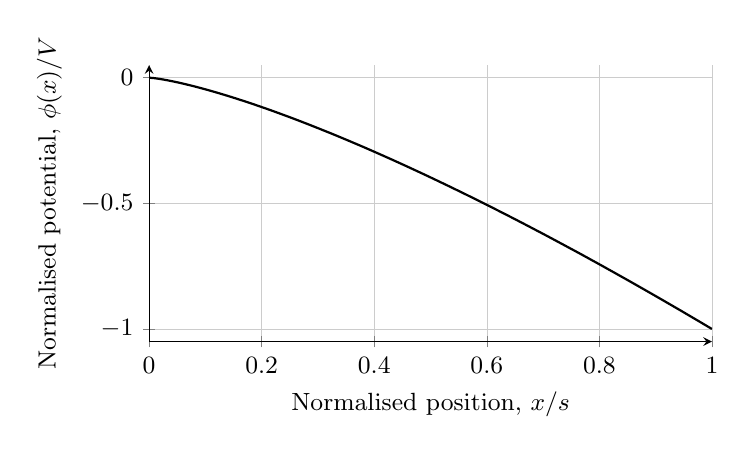
\begin{tikzpicture}
\begin{axis}[
 width=0.72\linewidth,
 height=0.42\linewidth,
 xlabel={Normalised position, $x/s$},
 ylabel={Normalised potential, $\phi(x)/V$},
 xmin=0, xmax=1,
 ymin=-1.05, ymax=0.05,
 domain=0:1,
 samples=100,
 axis lines=left,
 grid=both,
 grid style={line width=0.1pt, draw=gray!30},
 major grid style={line width=0.2pt, draw=gray!40},
 tick label style={font=\small},
 label style={font=\small},
 every axis plot/.append style={thick, black},
]
\addplot[black, thick] {-(x)^(4/3)};
\end{axis}
\end{tikzpicture}
\caption{Schematic potential profile of a planar, space-charge-limited (Child--Langmuir) sheath, plotted from the analytic law $\phi(x)/V=-(x/s)^{4/3}$ of Eq.~\eqref{eq:cl-profile}. No measured or simulated data are represented; the curve illustrates only the characteristic concave shape of the fluid-model sheath potential.}
\label{fig:cl-profile}
\end{figure}

\subsection{Where the fluid description breaks down}
\label{sec:breakdown}

The fluid sheath model is bounded by the same considerations as any truncated moment hierarchy: reliable when $f_{\mathrm{i}}(v)$ is sharply peaked and single-valued at each $x$, degrading when the distribution broadens, becomes multi-valued, or acquires trapped/reflected particles a single fluid velocity $u_{\mathrm{i}}(x)$ cannot represent. Four mechanisms drive this breakdown.

First, ions are not mono-energetic even at the sheath edge: born by ionisation across a spread of positions and accelerated by different potential drops, $f_{\mathrm{i}}(v)$ is a superposition with finite spread rather than a delta function. The Tonks--Langmuir kinetic model shows this spread is intrinsic to the collisionless presheath and irremovable by any scalar closure \cite{ref0665,ref0666}; the kinetic Bohm criterion, an integral condition on $f_{\mathrm{i}}(v)$, reduces to the fluid result only in the cold-beam limit and can differ materially near $v\to0$. Second, the density profile of Eq.~\eqref{eq:ni-of-phi} diverges as $u_{\mathrm{i}}(x)\to0$, avoided only because Eq.~\eqref{ch12-eq:bohm-criterion} guarantees $u_{\mathrm{i}}\ge u_{\mathrm{B}}>0$; a kinetic treatment instead lets the low-velocity tail vanish smoothly. Third, in magnetised or grazing-angle configurations ion gyromotion introduces velocity components a scalar or tensor closure captures only approximately; the Chodura magnetic presheath, acting over the ion gyroradius rather than the Debye length, is a multi-scale phenomenon fluid models reproduce only coarsely \cite{ref0017,ref0018}. Fourth, and most relevant here, the high-energy tail of the ion energy distribution — which sets sputtering-yield thresholds and etch/erosion-rate curves — is controlled by ions with atypical histories, invisible to a single-velocity cold-fluid closure, and needs either a fully kinetic solution or a fluid model augmented with a modelled energy spread \cite{ref0083}. Continuum-kinetic comparisons confirm the mean ion flux and leading Bohm moment are reproduced accurately by the fluid model, while higher moments — the energy-flux-weighted tail especially — deviate systematically as the ion thermal spread grows relative to the directed sheath-edge velocity \cite{ref0659}. In collisional or non-Maxwellian discharges, charge exchange repopulates low-energy ions throughout the sheath, producing a bimodal $f_{\mathrm{i}}(v)$ no single fluid velocity can represent without a multi-population closure \cite{ref0077,ref0090}.

\section{Boundary Conditions at the Sheath Edge}
\label{sec:bc}

\subsection{The Bohm criterion as a boundary condition}

In practice, the fluid sheath equations of Sec.~\ref{sec:sheath-models} are coupled to a quasineutral presheath solution from Sec.~\ref{sec:closure}, matched at a nominal "sheath edge." The Bohm criterion, Eq.~\eqref{ch12-eq:bohm-criterion}, is the boundary condition imposed there: the presheath must deliver ions with fluid velocity no smaller than $c_{\mathrm{s}}=\sqrt{T_{\mathrm{e}}/m_{\mathrm{i}}}$. The marginal equality is normally adopted, since the presheath field self-consistently accelerates ions to exactly $u_{\mathrm{B}}=c_{\mathrm{s}}$ where quasineutrality first fails; this is imposed as a Dirichlet-type velocity condition in essentially all fluid sheath codes.

\subsection{Generalised forms of the boundary condition}

Equation~\eqref{ch12-eq:bohm-criterion} generalises in several directions relevant to realistic discharges.

\begin{itemize}
\item \textbf{Warm and polytropic ions.} A finite ion temperature at the sheath edge raises the required entry speed to $u_{\mathrm{B}}=\sqrt{(T_{\mathrm{e}}+\gamma_{\mathrm{i}}T_{\mathrm{i}0})/m_{\mathrm{i}}}$ (Table~\ref{tab:closures}), applied as the boundary condition.
\item \textbf{Multiple ion species.} With two or more positive ion species of different mass, the criterion becomes an inequality on a weighted sum, $\sum_j n_{j}T_{\mathrm{e}}/(m_ju_j^2) \le n_{\mathrm{e}}$, so a light species may enter below its own sound speed if a heavier one compensates; individual boundary velocities need an auxiliary closure.
\item \textbf{Magnetised sheaths.} For a field inclined at angle $\alpha$ to the wall, the Bohm--Chodura condition requires the ion velocity along $\mathbf{B}$ to reach $c_{\mathrm{s}}$ at the magnetic presheath entrance, and the wall-normal component to satisfy the ordinary Bohm criterion at the thinner electrostatic sheath edge — two conditions at two distinct boundaries \cite{ref0017,ref0018}.
\item \textbf{Non-Maxwellian electrons.} If electrons deviate from Maxwellian, Eq.~\eqref{eq:boltzmann-electrons} no longer holds, and the boundary condition must be re-derived from the actual electron energy distribution, generally yielding a different coefficient in place of $\sqrt{T_{\mathrm{e}}/m_{\mathrm{i}}}$ \cite{ref0090}.
\end{itemize}

\subsection{Quasineutral matching and the presheath}

Formally, Eq.~\eqref{ch12-eq:bohm-criterion} is a marginal-stability condition on the quasineutral presheath solution, and the sheath itself is a boundary layer of thickness $\mathcal{O}(\lambda_{\mathrm{D}})$, thin compared with the presheath scale $\mathcal{O}(L)$. Matched-asymptotic treatments confirm the quasineutral presheath and non-neutral sheath equations can be solved as two separate problems, joined by continuity of $n_{\mathrm{i}}$, $u_{\mathrm{i}}$ and $\phi$ at the matching layer, with the Bohm criterion emerging as the solvability condition rather than an additional postulate. This is why a practical sheath code can patch a quasineutral drift-diffusion solution for the bulk onto a collisionless space-charge solution for the sheath, without resolving Debye-scale physics everywhere \cite{ref0012}.

\subsection{Practical implementation in fluid codes}

Three essentially equivalent implementations are common. The simplest fixes the ion fluid velocity at the last quasineutral grid point to the local sound speed, $u_{\mathrm{i}} = c_{\mathrm{s}}$, and integrates the sheath equations outward, adequate whenever the presheath solution is smooth. The second imposes a sonic outflow condition on the presheath drift-diffusion equation, letting the solution select where $u_{\mathrm{i}}$ first reaches $c_{\mathrm{s}}$, more self-consistent for non-planar geometries \cite{ref0013}. The third, used in particle and hybrid codes, replaces the sharp Bohm condition with a "logical sheath" or absorbing boundary that removes particles crossing a nominal wall and infers the sheath potential from the resulting charge imbalance, trading analytic transparency for validity when $f_{\mathrm{i}}(v)$ is not well approximated by a single fluid velocity (Sec.~\ref{sec:breakdown}) \cite{ref0659}. In all three, the presheath equations are solved up to where Eq.~\eqref{ch12-eq:bohm-criterion} is saturated, and the Sec.~\ref{sec:sheath-models} sheath solution is launched with $u_{\mathrm{i}}=u_{\mathrm{B}}$, $n_{\mathrm{i}}=n_{\mathrm{e}}=n_0$, $\phi=0$.

\section{Utility for Fast Forward Modelling in the Inversion}
\label{sec:forward}

\subsection{The computational cost hierarchy}

The inversion problem addressed by this monograph — recovering bulk plasma parameters ($n_0$, $T_{\mathrm{e}}$, and the sheath voltage or bias waveform) from a measured or targeted ion energy flux $\Gamma_E$ — requires a forward model evaluable an enormous number of times: once per proposal in a Markov-chain Monte Carlo sampler, once per grid-search combination, or once per optimiser iteration. Candidate forward models span many orders of magnitude in cost. A fully kinetic solution of Eq.~\eqref{ch12-eq:boltzmann} — by Vlasov discretisation, discontinuous-Galerkin methods, or particle-in-cell simulation with Monte Carlo collisions — requires resolving both the Debye length and electron plasma period, scaling unfavourably with the mass ratio $m_{\mathrm{i}}/m_{\mathrm{e}}$ and phase-space dimensionality. Continuum-kinetic solvers, though far more accurate than fluid models in the regimes of Sec.~\ref{sec:breakdown}, remain orders of magnitude more expensive per evaluation \cite{ref0659,ref0665,ref0666}. A single such solve, run once for validation, is tractable; running it inside an inversion with thousands to millions of calls is not.

\subsection{Semi-analytic ion energy flux from the fluid closure}

The fluid sheath model reduces the forward problem to evaluating a small number of closed-form or low-order-ODE expressions. Given $(n_0, T_{\mathrm{e}}, T_{\mathrm{i}0}, V_{\text{sheath}})$, the Bohm velocity follows from Table~\ref{tab:closures}; the sheath-edge flux from $\Gamma_{\mathrm{i}} = n_0u_{\mathrm{B}}$; and, in the cold-ion approximation, the ion energy flux at the wall from energy conservation along Eq.~\eqref{eq:ion-energy-cons} evaluated at $\phi=-V_{\text{sheath}}$,
\begin{equation}
\Gamma_E \simeq n_0u_{\mathrm{B}}\left(\tfrac{1}{2}m_{\mathrm{i}}u_{\mathrm{B}}^2 + eV_{\text{sheath}}\right),
\label{eq:GammaE-forward}
\end{equation}
a single algebraic expression, evaluable to machine precision in microseconds, replacing what would otherwise be a full kinetic transport calculation. Where the Child--Langmuir limit applies instead ($eV_{\text{sheath}}\gg T_{\mathrm{e}}$), Eq.~\eqref{ch12-eq:child-langmuir} gives an equally compact relation between voltage, sheath thickness and ion current density, from which $\Gamma_E \simeq J_{\mathrm{i}}V_{\text{sheath}}$ follows directly. Both expressions are low-order power laws, trivially differentiable in closed form, requiring no discretisation, mesh, or time-stepping.

\subsection{Role in the inversion workflow}

This monograph uses the fluid forward model of Eq.~\eqref{eq:GammaE-forward}, or its Child--Langmuir counterpart, as the workhorse evaluated inside the inversion loop, reserving kinetic or hybrid solves for a sparse set of validation points bounding the systematic error the closure introduces. This two-tier strategy is standard wherever cost asymmetry precludes a purely kinetic inversion: fast, closed-form fluid or power-balance relations serve parameter scans \cite{ref0093}, while more expensive models supply local corrections at limited anchor points. The bias from the cold-fluid closure — chiefly neglect of the ion energy spread (Sec.~\ref{sec:breakdown}) — can be partly compensated within the fluid framework by an energy-spectrum-resolved closure \cite{ref0083}, retaining a fluid solve's speed while approximating the leading kinetic correction. The fluid model of this chapter is thus not merely a pedagogical simplification but the load-bearing engine that makes a many-evaluation inversion of the ion energy flux problem feasible.

\section{Summary}

This chapter developed the fluid description of plasmas and sheaths as a systematic truncation of the moment hierarchy of the Boltzmann equation. The zeroth, first and second velocity moments gave continuity, momentum and energy equations~\eqref{eq:continuity}--\eqref{eq:energy}, an open hierarchy requiring an explicit closure. Cold, isothermal and polytropic pressure closures, the drift-diffusion reduction for collisional bulk plasmas, and the two-fluid model coupling ions and electrons through Poisson's equation were compared in Table~\ref{tab:closures}. The cold-ion, Boltzmann-electron closure applied to the collisionless planar sheath yielded the governing equation~\eqref{eq:sheath-ode}, from which the Bohm criterion, Eq.~\eqref{ch12-eq:bohm-criterion}, was derived by linear stability and the Sagdeev pseudopotential method, and the Child--Langmuir law, Eq.~\eqref{ch12-eq:child-langmuir}, obtained as the strongly biased limit. The Bohm criterion was then examined as the boundary condition coupling the quasineutral presheath to the non-neutral sheath, in its warm-ion, multi-species and magnetised generalisations, with practical implementation in fluid codes outlined. The chapter identified where the single-fluid-velocity closure breaks down — energy spread at the sheath edge, the apparent field singularity, magnetic presheath structure, and the high-energy distribution-function tail — and where a kinetic or hybrid treatment is necessary. Finally, via the closed-form Eq.~\eqref{eq:GammaE-forward}, it argued that reducing a phase-space kinetic problem to a handful of algebraic relations is what makes the fluid sheath model the appropriate forward operator for a many-evaluation inversion of ion energy flux measurements, with kinetic corrections retained only where Sec.~\ref{sec:breakdown} shows them necessary.
